\chapter{Marco Teórico}


En este capítulo se exponen los conceptos que explican el comportamiento de los datos y la suma importancia de conocer las características y comportamiento para hacer uso de los datos en la experimentación de este trabajo de tesis. Primero se habla sobre las \textit{series de tiempo} y las caracterísiticas que éstas deben cumplir para poder decir que estadísticamente los datos con los que contamos son útiles para la experimentación. Luego, se exponen los conceptos de \textit{autocorrelación}, \textit{autocovarianzas} y \textit{variograma}, y cómo estos conceptos ayudan a entender el comportamiento de los datos y a mejorar los resultados de la experimentación.

\section{Análisis Estadístico}

Se utilizan herramientas estadísticas para conocer el comportamiento de los datos, primero se usan series de tiempo para graficar los datos de contaminantes por estaciones y observar las características de éstas. Luego, se verifica si las series cumplen con la propiedad de ser estacionarias en el tiempo. Después se calcular los correlaciones y autocorrelaciones de los contaminantes por estación y por último, se calcula el variograma, el cual se utiliza como parámetro para encontrar el mejor método de interpolación de los métodos geoespaciales.

\subsection{Series de Tiempo}

Una \textit{serie de tiempo} es una secuencia cronológica de observaciones sobre una variable de interés \citep{montgomery}. Por ejemplo, la figura \ref{serie} muestra el rendimiento del mercado de los valores del tesoro de EE.\ UU.\ con vencimiento constante a 10 años desde abril de 1953 hasta diciembre de 2006. Este gráfico se llama \textit{diagrama de serie de tiempo}.

\begin{figure}[H]
\centering
\includegraphics[width=12cm, height=6cm]{./timeserie}
\caption{Gráfico de la serie de tiempo del rendimiento del mercado de valores del tesoro de EE.\ UU.\ con vencimiento constante a 10 años \citep{montgomery}}
\label{serie}
\end{figure}

Las mediciones de la variable de interés a estudiar se pueden recopilar en períodos de tiempo igualmente espaciados, como es típico en la mayoría de las series de tiempo. Los tiempos de recopilación pueden ser diarios, semanales, mensuales, trimestrales o anuales; pero se puede utilizar cualquier intervalo de tiempo, por ejemplo, en este trabajo las mediciones son hora a hora. Además, los datos pueden ser \textit{instantáneos}, como el nivel de un contaminante químico del aire en el momento en que se mide; \textit{acumulativo}, como las ventas totales de un producto durante un mes; o puede ser una \textit{estadística}, que de alguna manera refleja la actividad de la variable durante el período de tiempo.

La razón por la cual el registro de mediciones de una variable es tan importante se da porque la predicción de eventos futuros de dicha variable es un excelente aporte en muchos tipos de procesos de planificación y toma de decisiones, con aplicación en áreas como \citep{montgomery}:

\begin{itemize}
\item Márketing
\item Finanzas y gestión de riesgos
\item Ciencias económicas
\item Control de procesos industriales
\item Demografía
\end{itemize}

\subsection{Estacionariedad}

Un tipo importante de series de tiempo es una serie de tiempo \textit{estacionaria}. Se dice que una serie de tiempo es \textit{estrictamente estacionaria} si sus propiedades no se ven afectadas por un cambio en el origen del tiempo. Es decir, si la distribución de probabilidad conjunta de las observaciones $y_{t}, y_{t+1}, ..., y_{t+n}$ es exactamente la misma que la distribución de probabilidad conjunta de las observaciones $y_{t+k}, y_{t+k+1}, ..., y_{t+k+n}$, entonces la serie temporal es estrictamente estacionaria.

La figura \ref{serieene} (a) es un ejemplo de serie de tiempo estacionaria, ya que parece variar entorno a un nivel fijo, ésta es una característica de las series de tiempo estacionarias. Por otro lado, la figura \ref{serieene} (b) tiende a deambular a la deriva sin un nivel fijo obvio, este es un comportamiento típico de una serie de tiempo no estacionaria.

\begin{figure}[H]
\centering
\subfigure[Serie estacionaria \citep{montgomery}] {\includegraphics[width=70mm]{./seriee}}
\subfigure[Serie no estacionaria \citep{montgomery}]{\includegraphics[width=70mm]{./seriene}}
\caption{Series de tiempo}
\label{serieene}
\end{figure}

Cuando $n=0$, el supuesto de estacionariedad significa que la distribución de probabilidad de $y_{t}$ es la misma para todos los períodos de tiempo y puede escribirse como $f(y)$.

Estacionariedad implica un tipo de equilibrio estadístico o estabilidad en los datos \citep{montgomery}, es decir, la serie temporal tiene una media constante definida de la manera habitual como:
\begin{equation}
\mu_{y} = E[y] = \int_{- \infty}^{\infty} y f(y) dy,
\end{equation}

y la varianza constante definida como:
\begin{equation}
\sigma^{2}_{y} = \text{Var}[y] = \int_{- \infty}^{\infty} (y - \mu_{y})^{2} f(y) dy.
\end{equation}

La media muestral y la varianza muestral se utilizan para estimar estos parámetros. Si las observaciones en la serie de tiempo son $y_{1}, y_{2}, ..., y_{t}$, entonces la media muestral es:
\begin{equation}
\overline{y} = \hat{\mu}_{y} = \frac{1}{t} \sum_{t=1}^{t} y_{t},
\end{equation}

y la varianza muestral es:
\begin{equation}
s^{2} = \hat{\sigma}^{2}_{y} = \frac{1}{t} \sum_{t=1}^{t} (y_{t} - \overline{y})^{2}.
\end{equation}



\subsection{Autocovarianzas y Autocorrelaciones}

Si una serie de tiempo es estacionaria, esto significa que la distribución de probabilidad conjunta de cualquiera de las dos observaciones, por ejemplo, $y_{t}$ y $y_{t+k}$, es la misma para dos períodos de tiempo $t_{y}$ y $t_{t+k}$ que están separados por el mismo intervalo de tamaño $k$. El intervalo k se llama \textit{retraso}.

\begin{figure}[H]
\centering
\subfigure[Datos no correlacionados \citep{montgomery}] {\includegraphics[width=70mm]{./ncorr}}
\subfigure[Datos correlacionados \citep{montgomery}]{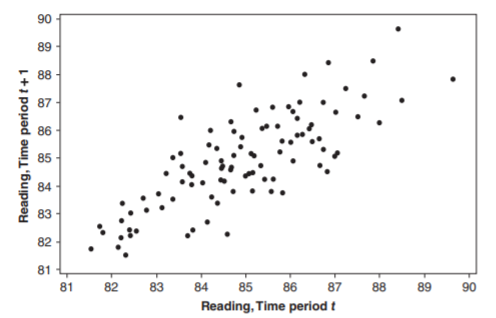
\includegraphics[width=70mm]{./corr}}
\caption{Datos correlacionados y no correlacionados}
\label{correlation}
\end{figure}

Las figuras \ref{correlation} (a) y \ref{correlation} (b) son diagramas de dispersión con un retraso $k=1$. Ambos diagramas de dispersión se construyeron trazando $y_{t+1}$ versus $y_{t}$. La figura \ref{correlation} (a)  exhibe poca estructura, ya que los pares trazados de observaciones adyacentes $y_{t}, y_{t+1}$ parecen no estar \textit{correlacionados}, es decir, el valor de $y$ en el período actual no proporciona ninguna información útil sobre el valor de $y$ que se observará en el próximo período. Por otro lado, en figura \ref{correlation}  (b), los pares de observaciones adyacentes $y_{t+1}, y_{t}$ están positivamente correlacionados, es decir, un valor pequeño de $y$ tiende a ser seguido en el siguiente período por otro valor pequeño de $y$, y un valor grande de $y$ tiende a ser seguido inmediatamente por otro valor grande de $y$.

La covarianza entre $y_{t}$ y su valor en otro período de tiempo, digamos, $y_{t+k}$ se llama \textit{autocovarianza} en el retraso $k$, definido por:
\begin{equation}
\gamma_{k} = \text{Cov}(y_{t},y_{t+k}) = E[(y_{t} - \mu)(y_{t+k} - \mu)].
\end{equation}

La colección de los valores de $\gamma_{k}$, $k = 0, 1, 2, ...$ se llama \textit{Función de autocovarianza}, donde la \textit{autocovarianza} en el retraso $k=0$ es la \textit{varianza} de la serie de tiempo, es decir, $\gamma_{0} = \sigma^{2}_{y}$, que es constante para una serie de tiempo estacionaria. Además, el coeficiente de autocorrelación en el intervalo $k$ para una serie temporal estacionaria se calcula como:
\begin{equation}
\rho_{k} = \frac{E[(y_{t} - \mu)(y_{t+k} - \mu)]}{\sqrt{E[(y_{t} - \mu)]^{2} E[(y_{t+k} - \mu)^{2}]}} = \frac{\text{Cov}(y_{t},y_{t+k})}{\text{Var}(y_{t})} = \frac{\gamma_{k}}{\gamma_{0}}.
\end{equation}

La colección de los valores de $\rho_{k}$, $k = 0, 1, 2, ...$ se llama \textit{Función de autocorrelación (ACF)}, donde $\rho_{0} = 1$. Además, el ACF es independiente de la escala de medición de la serie de tiempo. También, $\rho_{k} = \rho_{-k}$, es decir, el ACF es simétrico alrededor de cero, por lo que solo es necesario calcular la mitad positiva (o negativa).

Si una serie de tiempo tiene función de autocovarianza y media finita, se dice que es estacionaria de segundo orden (o débilmente estacionaria de orden dos). Si además, la distribución de probabilidad conjunta de las observaciones en todo momento es multivariante normal, entonces eso es suficiente para dar como resultado una serie de tiempo estrictamente estacionaria.

Es necesario estimar la autocovarianza y los ACF a partir de un momento de longitud finita, digamos, $y_{1}, y_{2}, ..., y_{t}$. La estimación habitual de la función de autocovarianza se calcula como:
\begin{equation}
c_{k} = \hat{\gamma_{k}} = \frac{1}{T} \sum_{t=1}^{T-k} (y_{t}-\overline{y})(y_{t+k}-\overline{y}), \ k=0, 1, ..., k,
\end{equation}

y el ACF es estimado por la función de autocorrelación de muestra (o muestra de ACF) calculada como:
\begin{equation}
r_{k} = \hat{\rho_{k}} = \frac{c_{k}}{c_{0}}, \ k=0, 1, ..., k.
\end{equation}

\subsection{Variograma}

A menudo en la práctica no hay una demarcación clara entre un proceso estacionario y uno no estacionario para muchas series de tiempo del mundo real. Por ello, una herramienta de diagnóstico adicional que es muy útil es el \textit{Variograma}.

Suponga que las observaciones de la serie de tiempo están representadas por $y_{t}$. El variograma $G_{k}$ mide las variaciones de las diferencias entre las observaciones que están separadas a una distancia $k$, en relación con la variación de las diferencias que están separadas por una unidad de tiempo. El variograma se define como:
\begin{equation}
G_{k} = \frac{\text{Var}(y_{t+k}-y_{t})}{\text{Var}(y_{t+1}-y_{t})}, k=1, 2, ...
\end{equation}

y los valores de $G_{k}$ se representan en función del retraso $k$. Si la serie temporal es estacionaria, resulta que:
\begin{equation}
G_{k} = \frac{1- \rho_{k}}{1-\rho_{1}},
\end{equation}

para una serie temporal estacionaria $\rho_{k} \rightarrow 0$ a medida que $k$ aumenta, por lo que cuando el variograma se traza contra el retraso $k$, $G_{k}$ alcanzará una asíntota $\frac{1}{(1 - \rho_{1})}$. Sin embargo, si la serie temporal no es estacionaria, $G_{k}$ aumentará monótonamente. 



\section{Métodos de Interpolación}

Sea $P_{n} = \{ p_{1}, p_{2}, ..., p_{n} \}, n \geq 2$ el conjunto de puntos muestrales (estaciones de monitoreo) en el espacio $\mathbb{R}^{2}$ o \textit{plano Euclideano}, etiquetados mediante las coordenadas $(x_{1}, y_{1}), ..., (x_{n}, y_{n})$. Los $n$ puntos son distintos en el sentido de que $(x_{i}, y_{i}) \neq (x_{j}, y_{j}) \ \forall p_{i}, p_{j} \in P_{n}$.


\begin{defn} \textbf{(Distancia Euclidiana)}. Sean $p$ y $p^{*}$ dos puntos arbitrarios en el plano Euclidiano con coordenadas $(x, y)$ y $(x^{*}, y^{*})$ respectivamente. Entonces, la \textit{distancia Euclidiana} entre $p$ y $p^{*}$ está dada por:
\begin{equation}
d(p, p^{*}) = \lVert p - p^{*} \rVert = \sqrt{ {(x-x^{*})}^{2} + {(y-y^{*})}^{2} }.
\end{equation} \end{defn}

\textbf{Nota:} Se considera a partir de ahora que se trabaja en el espacio Euclidiano con la \textit{métrica Euclidiana}.


\subsection{Determininistas}

La interpolación mediante métodos de interpolación deterministas indica los valores de un punto desconocido a través de una combinación ponderada linealmente de un conjunto de puntos conocidos (puntos de muestra). Los métodos de interpolacion deterministas suponen que la superficie que se interpola debe ser la de una variable dependiente de la ubicación. En esta sección se definen los métodos de interpolación deterministas que se utilizan en este trabajo y son: Diagramas de Voronoi, Funciones de Base Radial y el método de Distancia Inversa Ponderada.

\subsubsection{Diagramas de Voronoi}


\begin{defn} \textbf{(Diagrama de Voronoi (DV))}. Sea el conjunto $P_{\mathcal{V}}$ = $\{ p_{1}, p_{2}, ...,$ \\ $p_{n} \} \subset \mathbb{R}^{2}$, con $2 < n$ y $x_{i} \neq x_{j} \forall \ i, j$. Llamemos a la región dada por: 
\begin{equation}  
V(p_{i})= \{x : \parallel x-x_{i} \parallel \leq \parallel x-x_{j} \parallel, i \neq j \} \ \forall x_{i}, x_{j} \in P_{\mathcal{V}},
\label{pol_voronoi}
\end{equation}
como el \textit{Polígono de Voronoi} asociado a $p_{i}$ (o el Polígono de Voronoi de $p_{i}$ y al conjunto dado por
\begin{equation}
\mathcal{V} = \{ V(p_{1}),...,V(p_{n}) \}
\end{equation}
el \textit{Diagrama de Voronoi} generado por $P_{\mathcal{V}}$ (o el diagrama de Voronoi de $P_{\mathcal{V}}$). 
\label{voronoi}
\end{defn}

En la definición \ref{voronoi}, se observa de la ecuación \ref{pol_voronoi} que está definida en términos de desigualdad $(\leq)$, por lo que un polígono de Voronoi es un \textit{conjunto cerrado}. Dado que un polígono de Voronoi, éste contiene su frontera ($\partial V(p_{i})$) y podemos establecer las siguientes definiciones.

\begin{defn} \textbf{(Arista de Voronoi)}. Puesto que el diagrama de Voronoi contiene a su frontera $\partial V(p_{i})$, ésta puede consistir en segmentos de recta, semirectas o rectas infinitas, las cuales llamamos \textit{Aristas de Voronoi}. Denotamos a la arista de los polígonos de Voronoi $p_{i}$ y $p_{j}$ como $a (p_{i}, p_{j})$.
\end{defn}

\begin{defn} \textbf{(Vértice de Voronoi)}. Llamamos \textit{Vértice de Voronoi} a un punto extremo de una arista de Voronoi o se puede definir también como un punto compartido por tres o más polígonos de Voronoi. Denotamos a el vértice de Voronoi del polígono de Voronoi $p_{i}$ como $v_{i}$.
\end{defn}

\begin{defn} \textbf{(Red de Voronoi)}. El diagrama de Voronoi puede ser definido por la unión de las aristas de Voronoi, es decir, $\bigcup_{i=1}^{n} \partial V(p_{i})$  en lugar del conjunto $P_{\mathcal{V}}$. Llamamos a red \textit{(malla)}, conformada por la unión de aristas de Voronoi como la \textit{Red de Voronoi}.
\end{defn}





\subsubsection{Funciones de base radial}


\begin{defn} \textbf{(Funciones de Base Radial (FBR))}. Sea el conjunto $P_{\mathcal{F}} = \{ p_{1}, p_{2}, ..., p_{n} \} \subset \mathbb{R}^{2}$, con $x_{i} \neq x_{j} \forall \ i, j$. Llamemos \textit{Función de Base Radial} a una función perteneciente a una gran familia de interpoladores exactos que usan una \textit{ecuación básica} que es una función que depende de la distancia entre el punto interpolado y los puntos de muestreo $P_{\mathcal{F}}$. Los valores de predicción por una FBR se pueden expresar como la suma de dos componentes: 
\begin{equation} 
\hat{Z}(x)=\sum_{i=1}^{n} a_{i} f_{i}(x) + \sum_{j=1}^{n} b_{j} \psi(d_{j}), 
\end{equation}
donde $\psi(d_{j})$ es la ecuación básica que depende de la distacia $d_{j}$, donde $d_{j}$ es la distancia desde los puntos de muestra $P_{\mathcal{F}}$ a el punto interpolado $x$ y $f_{i}(x)$ es un polinomio de grado $< m$, con $m$ el número de puntos a interpolar. Los coeficientes $a_{i}$ y $b_{j}$ se calculan mediante la resolución del sistema de $n + m$ ecuaciones lineales, con $n$  el número de puntos conocidos $P_{\mathcal{F}}$ utilizados en la interpolación de la siguiente manera:
\begin{equation}
\hat{Z}(x_{k}) = \sum_{i=1}^{m} a_{i} f_{i}(x_{k}) + \sum_{j=1}^{n} b_{j} \psi(d_{jk}), \ k=1, 2, ..., n 
\end{equation}
\[ \sum_{j=1}^{n} b_{j} f_{k}(x_{j}) = 0, \ k= 1, 2, ..., m. \]
\end{defn}

En este trabajo de tesis se utilizan las siguientes clases de BRF para la interpolación de datos dispersos $n$-dimensionales a un dominio $m$-dimensional; Multicuadrática (M), Inversa multicuadrática (IM), Gaussiana (G), Lineal (L), Cúbica (C), Quíntica (Q) y Thin-plate splines (TPS). La función de base radial utilizada para cada caso da las siguientes expresiones:
\begin{itemize}
\item M: $\psi(d) = \sqrt{d^{2} + c^{2}}$
\item IM: $\psi(d) = \sqrt{d^{2} + c^{2}}^{-1}$
\item G: $\psi(d) = e^{-\sqrt{d^{2} + c^{2}}}$
\item L: $\psi(d) = d$
\item C: $\psi(d) = d^{3}$
\item Q: $\psi(d) = d^{5}$
\item TPS: $\psi(d) =  d^{2} + c^{2} \ln (cd)$,
\end{itemize}

donde $d$ es la distancia de los puntos muestra $P_{\mathcal{F}}$ a la ubicación de predicción $x$ y $c$ es un factor de suavizado.






\subsubsection{Distancia inversa ponderada}



\begin{defn} (\textbf{Distancia Inversa Ponderada (DIP)}). Sea el conjunto $P_{\mathcal{D}} = \{ p_{1}, p_{2}, ..., p_{n} \} \subset \mathbb{R}^{2}$, con $x_{i} \neq x_{j} \forall \ i, j$. Llamemos función de \textit{Distancia Inversa Ponderada} a una función de la forma:
\begin{equation}
\hat{Z}(x)= \frac{\sum_{i=1}^{n} w_{i}z_{i}}{\sum_{i=1}^{n} w_{i}}
\end{equation}
\[ w_{i}=d_{i}^{-u}, \]
donde $Z(x)$ es el valor predicho en el punto $x$, $Z_{i}$ es el valor del punto muestra $p_{i}$, $d_{i}$ es la distancia entre el punto $p_{i}$ y el punto $x$ y $w_{i}$ es el peso asignado al punto $p_{i}$.
\end{defn}

Los valores de mayor ponderación se asignan a valores más cercanos al punto interpolado. A medida que la distancia aumenta, el peso disminuye \citep{shepard}, y $u$ es el poder de ponderación que decide cómo disminuye el peso a medida que aumenta la distancia.





\subsection{Geoestadísticos}

La interpolación mediante métodos de interpolación geoestadísticos o probabilísticos se resumen en el método de interpolación \textit{Kriging}. La palabra Kriging (expresión anglosajona) proviene del nombre del geólogo sudafricano Danie G. Krige, cuyo trabajo aportó a la predicción de reservas de oro, realizados en la década de los años cincuentas y éste suele considerarse como el pionero en los métodos de interpolación geoespacial. 

Kriging encierra un conjunto de métodos de predicción espacial que se centran en la minimización del error cuadrático medio de predicción. Al igual que con DIP, el estimador de Kriging viene dado por una combinación lineal de los valores observados y los pesos. Dependiendo de las propiedades estocásticas de los campos aleatorios, se aplican diferentes tipos de Kriging. En esta sección se definen los métodos de interpolación geoestadísticos que se utilizan en este trabajo y son: Kriging Ordinario y Kriging Universal.



\subsubsection{Kriging Ordinario}

\begin{defn} (\textbf{Kriging Ordinario (KO)}). Sea el conjunto $P_{\mathcal{O}} = \{ p_{1}, p_{2}, ..., p_{n} \} \\ \subset \mathbb{R}^{2}$, con $x_{i} \neq x_{j} \forall \ i, j$. Supongase que se hacen mediciones de la variable de interés $Z$ en los puntos $p_{i} \in P_{\mathcal{O}} \forall i$, es decir, se tienen $Z(x_{1}), ..., Z(x_{n})$, y se desea predecir el punto $Z(x^{*})$, en el punto $x^{*}\notin P_{\mathcal{O}}$ donde no hubo medición. Llamemos \textit{Kriging Ordinario} al método que predice con una combinación lineal las $n$ variables aleatorias como:
\begin{equation}
\hat{Z}(x^{*}) = \lambda_{1} Z(x_{1}) + \lambda_{2} Z(x_{2}) + ... + \lambda_{n} Z(x_{n}) = \sum_{i=1}^{n} \lambda_{i} Z(x_{i}), \end{equation} donde $\lambda_{i}$ representan los pesos de los valores de los puntos muestrales y $x_{i}$ son los valores observados en los puntos $p_{i}$.
\end{defn}

Dichos pesos se calculan en función de la distancia entre los puntos muestrales $(P_{\mathcal{O}})$ y el punto predicho $x^{*}$. La suma de los pesos debe ser igual a uno para que la esperanza del predictor sea igual a la esperanza de la variable. Esto último se conoce como \textit{propiedad de insesgamiento}. 

Estadísticamente la propiedad de insesgamiento es:
\[ E\left[ \sum_{i=1}^{n} \lambda_{i} Z(x_{i}) \right] = m, \]
\[ \sum_{i=1}^{n}  \lambda_{i} E[Z(x_{i})] = m, \]
\[ \sum_{i=1}^{n}  \lambda_{i} m = m, \]
\[m \sum_{i=1}^{n}  \lambda_{i} = m \Rightarrow \sum_{i=1}^{n}  \lambda_{i} = 1.\]

Se dice que $\hat{Z}(x^{*})$ es el mejor predictor lineal en este caso, ya que los pesos se obtienen de tal manera que minimicen la varianza del error de predicción, es decir, que minimicen la expresión dada por:
\begin{equation}
V[ \hat{Z}(x^{*}) - Z(x^{*})].
\end{equation}
Esta característica es distintiva de los métodos Kriging, ya que métodos de interpolación deterministas no garantizan
varianza mínima de predicción \citep{samper}. La estimación de los pesos se obtiene resolviendo:
\[\text{Min.} \ \ V[ \hat{Z}(x^{*}) - Z(x^{*})] \]
\[ \text{s. a.} \ \ \sum_{i=1}^{n}  \lambda_{i} = 1. \] 


Los pesos de KO se derivan de la \textit{función de semivariancia}. Los parámetros de la función de semivariancia y el \textit{efecto de pepita} se pueden estimar mediante una \textit{función de semivariación empírica} \citep{webster}. Un estimador imparcial de la función de semivariancia es la mitad de la diferencia cuadrática promedio entre los valores de datos dado por:
\begin{equation}
\gamma (h) = \frac{1}{2N(h)} \sum_{i=1}^{N(h)} [z(x_{i}) - z(x_{i} +h)]^{2}, 
\end{equation}
donde $\gamma (h)$ es el valor de semivariancia en el intervalo de distancia $h$, $N(h)$ es el número de pares de muestras dentro del intervalo de distancia $h$ y $z(x_{i} + h)$ y $z(x_{i})$ son valores de muestra en dos puntos separados por el intervalo de distancia $h$.




\subsubsection{Kriging Universal}

En los supuestos de KO se ha asumido que la variable es estacionaria, pero en la mayoría de los casos la variable no satisface esta condición y se caracteriza por exhibir una tendencia. Para tratar este tipo de variables es frecuente descomponer la variable $Z(x)$ en la suma de la tendencia, tratada como una función determinística más una componente estocástica estacionaria de media cero.

\begin{defn} (\textbf{Kriging Universal (KU)}). Sea el conjunto $P_{\mathcal{U}} = \{ p_{1}, p_{2}, ..., p_{n} \} \subset \mathbb{R}^{2}$, con $x_{i} \neq x_{j} \forall \ i, j$. Llamemos \textit{Kriging Universal} al método que predice como la suma de la tendencia, tratada a manera de una función determinística más una componente estocástica estacionaria de media cero las $n$ variables aleatorias, por ejemplo:
\begin{equation}
\hat{Z}(x) = m(x) + \epsilon(x),
\end{equation}
con $E[\epsilon(x)] = 0$, $V[\epsilon(x)] = \sigma^{2}$ y $E[Z(x)] = m(x)$.
\end{defn}

La tendencia puede expresarse mediante:
\[ m(x) = \sum_{l=1}^{p} a_{l} f_{l} (x), \]
donde las funciones $f_{l}(x)$ son conocidas y $p$ es el número de términos empleados para ajustar $m(x)$. Por lo tanto, el predictor de KU se define como:
\begin{equation}
\hat{Z} (x^{*}) = \sum_{i=1}^{n} \lambda_{i} Z(x_{i}).
\end{equation} 

 
























